This section contains four parts.
%
Section~\ref{sec:insituinfrastructure} describes the in situ infrastructure for our approaches.
%
The next two sections describe the two Lagrangian flow map extraction approaches:
the traditional approach~(\ref{sec:baseline}) and a new communication-free approach~(\ref{sec:local}).
Section~\ref{sec:posthoc} describes how post hoc reconstruction, which applies to both approaches, is performed.
%
Further, based on the in situ system classification in~\cite{childs2020istp}, the Lagrangian flow map extraction system is classified as one with a dedicated API integration, on node proximity, direct access, a time division of execution, automatic operation, and a derived output type.

%\vspace{-2mm}
\subsection{In Situ Infrastructure}
\label{sec:insituinfrastructure}
\begin{figure}[!b]
\centering
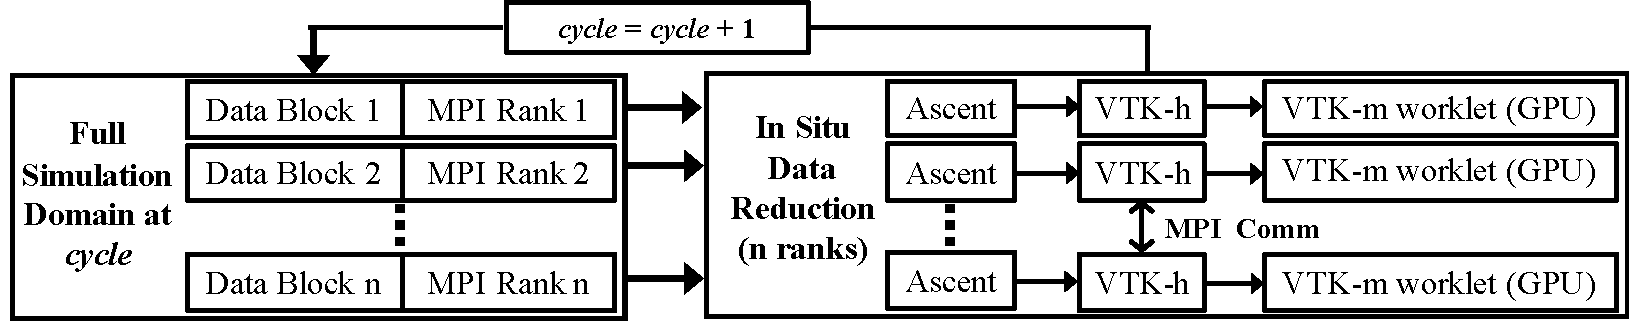
\includegraphics[width=\linewidth]{Images/insitu_infrastructure_flat.pdf}
\caption{Workflow of in situ data reduction distributed across \textit{n} processes to compute a Lagrangian flow map.}
\label{fig:insituinfrastructure}
\end{figure}

Our study used the Ascent in situ infrastructure~\cite{Larsen2017Ascent}.
%
The Ascent API can be used to integrate with a simulation code and access various in situ analytics capabilities.
%
It can also be used to create a workflow when loading data sets from disk.
%
The fundamental operation of particle advection required to compute the particle trajectories that form the Lagrangian flow map is implemented using the VTK-m library~\cite{moreland2016vtk}.
%
VTK-m is a platform-portable scientific visualization library for shared-memory parallel environments and enabled us to easily engage GPUs for particle advection.
%
Specifically, we used a fourth-order Runge Kutta interpolation implemented as a VTK-m worklet~\cite{pugmire2018performance}.
%
Ascent has VTK-h~\cite{Larsen2017Ascent} as a distributed-memory wrapper around VTK-m.
%
VTK-h uses MPI and acts as the communication layer.
%
Figure~\ref{fig:insituinfrastructure} provides an illustration of the workflow for in situ data reduction.
%
Ascent is invoked every cycle of the simulation, and it consequently invoked the relevant calls to the Lagrangian \textit{filter} (VTK-h + VTK-m).
%
The rank-specific Lagrangian filter used the simulation vector field data to advect particles every cycle, and triggered the storage of trajectories that comprise the Lagrangian flow map. 
%
%Creating an instance of Ascent, specifying parameters, and invoking the Lagrangian filter requires only 20 lines of code (C++) and fewer if a JSON input file is used.


\begin{figure*}[!ht]
\begin{subfigure}{0.16\textwidth}
\centering
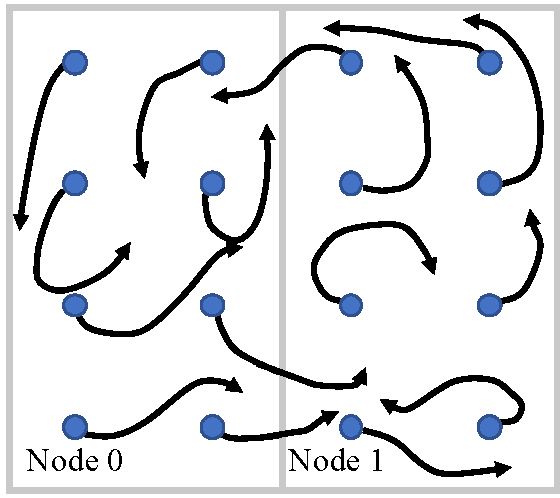
\includegraphics[width=\linewidth]{Images/notion_dist_1.pdf}
\caption{}
\label{fig:dist_1}
\end{subfigure}
\begin{subfigure}{0.16\textwidth}
\centering
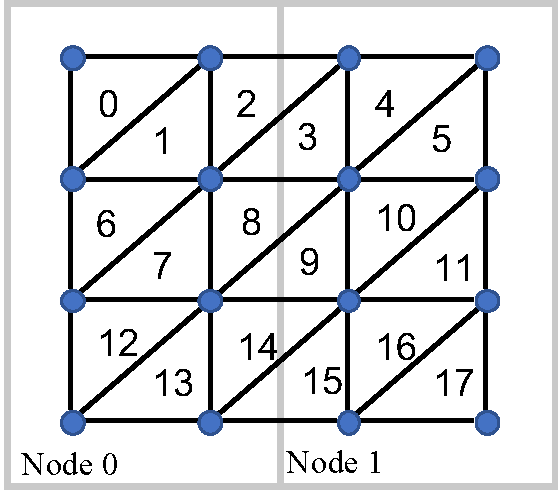
\includegraphics[width=\linewidth]{Images/notion_dist_2.pdf}
\caption{}
\label{fig:dist_2}
\end{subfigure}
\begin{subfigure}{0.16\textwidth}
\centering
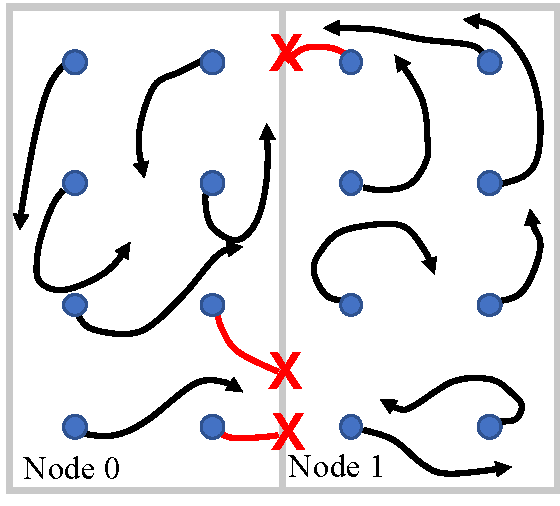
\includegraphics[width=\linewidth]{Images/notion_local_1.pdf}
\caption{}
\label{fig:local_1}
\end{subfigure}
\begin{subfigure}{0.16\textwidth}
\centering
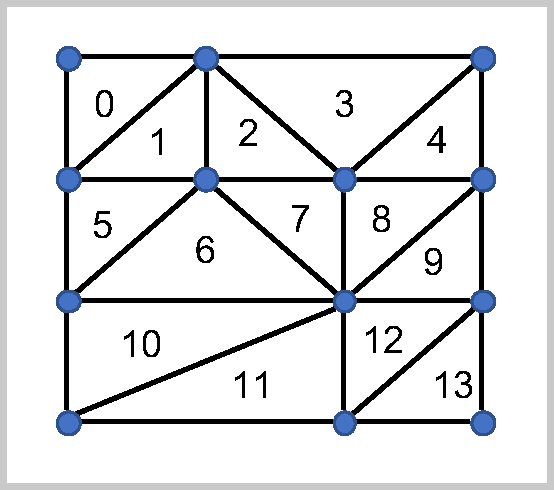
\includegraphics[width=\linewidth]{Images/notion_local_2.pdf}
\caption{}
\label{fig:local_2}
\end{subfigure}
\hfill
\begin{subfigure}{0.34\textwidth}
\centering
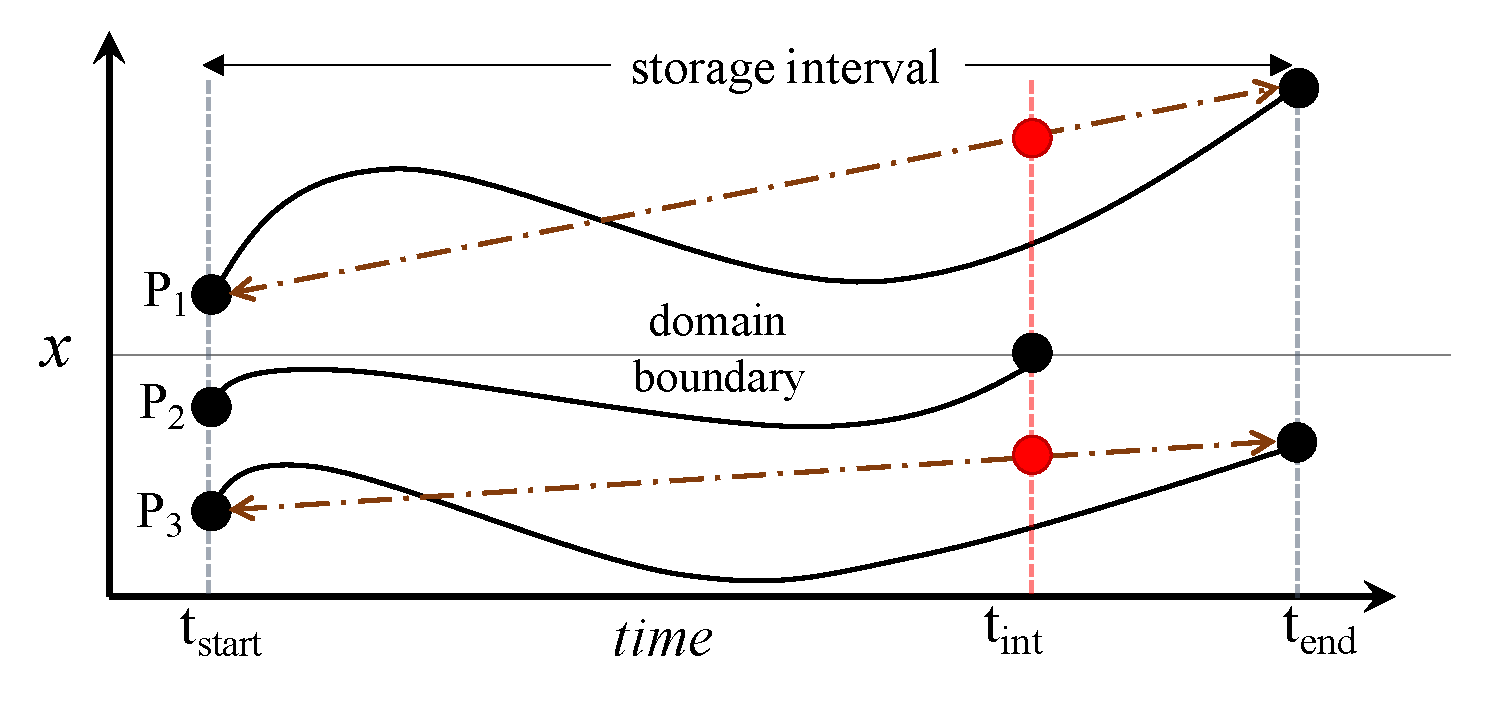
\includegraphics[width=\linewidth]{Images/early_termination.pdf}
\vspace{-8mm}
\caption{}
\label{fig:early_termination}
\end{subfigure}
\caption{\fix{Figures~\ref{fig:dist_1} and~\ref{fig:local_1} notionally illustrate the in situ computation of Lagrangian$_{Dist}$ and Lagrangian$_{Local}$ flow maps, respectively. Figures~\ref{fig:dist_2} and~\ref{fig:local_2} show the corresponding global Delaunay triangulations~(see Section~\ref{sec:posthoc} for details of post hoc reconstruction). Figure~\ref{fig:early_termination} illustrates a case of early termination, which is discussed in Section~\ref{sec:local}.}}
%\caption{The examples demonstrate in situ computation and post hoc use of Lagrangian$_{Dist}$~(\ref{fig:dist_1},~\ref{fig:dist_2}) and Lagrangian$_{Local}$(\ref{fig:local_1},~\ref{fig:local_2}) flow maps.}
\vspace{-4mm}
\label{fig:notional_examples}
\end{figure*}


%\vspace{-2mm}
\subsection{Traditional Computation of Lagrangian Flow Maps}
\label{sec:baseline}
Conceptually, a Lagrangian representation encodes the behavior of a time-varying flow using particle trajectories.
%
Given the early nature of investigations into the use of Lagrangian flow maps, the best ways to seed, represent in memory, communicate, and store flow maps are open questions. 
%
%Prescribing the optimal approach to sample a four-dimensional space in a distributed-memory in situ setting is challenging and can vary based on the nature of the vector field.
%
Section~\ref{sec:related} noted three prior sampling strategies; however, none of these were evaluated at scale.
%
As a baseline, our work implemented the technique described by Agranovsky et al.~\cite{agranovsky2014improved}
% with a modification to the storage format. 
%
and is referred to as Lagrangian$_{Dist}$.

For Lagrangian$_{Dist}$, we defined the overall strategy for flow map computation by considering four aspects:
%
\begin{itemize}[leftmargin=*]
\item\textbf{Sampling:} For each data block, seeds are placed along a uniform grid. As particles are advected, they may diverge or cluster. 
%
To maintain domain coverage, particles are terminated after a fixed number of cycles, i.e., storage interval, and their end locations are saved, followed by a new set of particles uniformly seeded at the original starting locations.
%
Thus, sets of temporally non-overlapping particle trajectories are calculated that span the full duration of the simulation.
%
\item\textbf{In-memory Representation:} %Particle trajectories can be represented in various forms. 
%
Adopting a minimal approach, only the current location and the validity of the particle are statically stored in memory. 
%
\item\textbf{Communication:} Ranks communicated every cycle to check for particles (incoming/outgoing) crossing rank boundaries to continue trajectory integration. 
%\item\textbf{Communication:} Ranks communicate every cycle to check whether any particles are incoming and to send particles that need to cross rank domain boundaries to continue trajectory integration. 
%
Control is returned to the simulation after all communication is completed.
\item\textbf{Storage:} Agranovsky et al. did not specify how particles that exited the domain before the end of the storage interval are saved,
%
which is problematic for post hoc reconstruction. 
%
In our implementation, we stored the end location and a Boolean indicating validity, i.e., whether the particle remained within the domain for the entirety of the storage interval. 
%
%Prior to storage, particles that have traveled across boundaries are communicated back to the originating rank. 
%
\end{itemize}

%From a performance perspective, 
%Our focus in this work is the execution time for computing a Lagrangian flow map.
%
\fix{Is this paragraph needed? The particle advection workload and interprocess communication impact the execution time.
%
%Performing an advection step involves transferring the current vector field slice to GPU memory and invoking the advection kernel on each cycle.
%
The cost of particle advection depends on the data set, number of particles that each GPU is operating on, and the number of GPUs sharing memory on a CN.
%
Communication involves exchanging particle information and synchronization. 
%
The cost of communication varies based on the number of CNs, the number of total ranks, rank distribution across CNs, and the number of particles exchanged.
%
Finally, we considered the minimal encumbrance that can be placed on runtime memory for this technique: storing only current location and validity, and accessing only the vector field needed for a single step at any given time.}
%
%a single vector field time-slice at any given time.
%
%\vspace{-2mm}
\subsection{Computation of Local Lagrangian Flow Maps}
\label{sec:local}
%As mentioned in the previous section, the two main costs are (1) an advection step and (2) communication.
%
%Performing an advection step involves transferring the current vector field slice to GPU memory and invoking the advection kernel on each cycle.
%
%Then, the cost of particle advection depends on the number of particles that each GPU is operating on and the number of GPUs sharing memory on a CN.
%
%Communication involves exchanging particle information and synchronization. 
%
%The cost of communication varies based on the number of CNs, the number of total ranks, the number of ranks on each CN, and the number of particles exchanged.
%
With this work, we propose an optimization to address the increasing cost of communication as the scale increases.
%
Our strategy is a simple, yet novel and scalable, approach: skip all the communication and compute only local Lagrangian flow maps in situ. 
%
We refer to this implementation as Lagrangian$_{Local}$ and define the overall strategy as follows:
\begin{itemize}[leftmargin=*]
\item\textbf{Sampling:} Similar to Lagrangian$_{Dist}$, we used a uniform seed placement and a fixed storage interval.
%
Further, seeds can be placed redundantly along domain boundaries in adjacent ranks, and although our study does not consider ghost zones, we believe these would serve to strengthen our proposed optimization.
%
\item\textbf{In-memory representation:} Similar to Lagrangian$_{Dist}$, we stored the current location and validity of a particle.
%
\item\textbf{Communication:} We eliminated all particle information exchange and synchronization. Particles that required communication to continue trajectory integration are discarded. Thus, all ranks operated independently.
%
\item\textbf{Storage:} For a uniform grid, we stored the end location (3 double) and validity (1 Boolean). Particles that are discarded were marked as invalid. 
%
\end{itemize}

%Figures~\ref{fig:dist_1} and~\ref{fig:local_1} show notional examples of the particle trajectory calculation for Lagrangian$_{Dist}$ and Lagrangian$_{Local}$, respectively. 
%
An interesting consideration was whether to store the particle location and time of termination on the domain boundary.
%
Figure~\ref{fig:early_termination} illustrates the problem with this approach.
%
The diagram shows three particle trajectories (P$_{1}$, P$_{2}$, P$_{3}$) starting at time t$_{start}$.
%
Two of the particle trajectories (P$_{1}$, P$_{3}$) remain in their domain until t$_{end}$, i.e., for all cycles of the storage interval, and one particle (P$_{2}$) reaches the domain boundary at t$_{int}$.
%
During post hoc reconstruction, using the information of P$_{2}$ to transport a new particle from t$_{start}$ to t$_{int}$ requires knowing the location of neighboring particles (P$_{1}$, P$_{3}$) at t$_{int}$.
%
Only the start and end locations of the particles are known in our case, so this approach would require linearly interpolating (depicted using the dotted brown line) the locations of the neighboring particles at t$_{int}$.
%
However, these interpolated locations are often errorneous (red particles).
%
%Further, using such information can result in a particle taking many small steps to reach the end of the storage interval.
%
%We discuss a potential strategy to address this in Section~\ref{sec:discussion}.

The benefits of computing local Lagrangian flow maps are reduced execution time and improved scalability characteristics. 
%
Further, for storage intervals that are used in practice, we hypothesize only a small percentage of particles will be discarded.
%
However, the loss of information in the form of discarded particle trajectories could reduce the quality of flow reconstruction.
%
Discarded or new trajectories can be interpolated using valid trajectories from adjacent processors during post hoc analysis.
%
Our study evaluates this tradeoff.
%
Lastly, we believe this performance optimization could be applied adaptively, i.e., communication can be turned on/off when appropriate.
%
Our study assumed an ``always off'' approach, which we view as invaluable for future adaptive designs.
%That said, we view this study as essential to inform such heuristic design. % and leave it for future work.
%
%In this paper, we treat the computation of local Lagrangian flow maps as a separate technique to understand behavior across every stage of a simulation run.
%
%We refer to our implementation of local Lagrangian flow maps as Lagrangian$_{Local}$.

%\vspace{-2mm}
\subsection{Post Hoc Flow Field Reconstruction}
\label{sec:posthoc}
We used a Lagrangian-based advection scheme similar to prior work~\cite{agranovsky2014improved, sane2018revisiting, sane2019interpolation}.
%
New particles interpolate temporally nonoverlapping sets of particle trajectories, with an advection step advancing the particle forward in time by the length of the storage interval.
%
%Our implementation considers a simple parallelize-over-data strategy with data duplication. 
%
%Each processor loads a primary data block and the particle trajectories from adjacent ranks.
%
%On a processor, for particle trajectories encoding a specific storage interval, 
%
For a specific storage interval, the starting positions of all valid trajectories are treated as points in an unstructured mesh.
%
To calculate the trajectory of a particle $P$, the \textit{neighborhood}, i.e., the containing cell of the unstructured mesh, is first identified.
%
We computed the cells of the unstructured mesh by performing Delaunay triangulation.
%
%Figures~\ref{fig:dist_2} and~\ref{fig:local_2} illustrate examples of the triangulation for Lagrangian$_{Dist}$ and Lagrangian$_{Local}$, respectively. 
%
%To accelerate neighborhood identification, we consider local Delaunay triangulations.
%
%To advect particles within a specific block, the points for the block itself as well as points from every adjacent block are considered in the triangulation.
%
%For example, to advect particles in the domain of rank A, the flow maps extracted from rank A and all of its adjacent ranks are used to compute a local Delaunay triangulation.
%
%An assumption here is that a sufficiently good approximation of the global Delaunay triangulation can be made for cells within the primary block if points of every adjacent block are included in the triangulation.
%
The identified neighborhood forms a convex hull around the particle $P$.
%
Next, $P$ ``follows'' the neighborhood until the end of the specific storage interval.
%
To compute the next location of $P$, we used the end locations of the neighborhood particles and barycentric coordinate interpolation as suggested by Agranovsky et al.~\cite{agranovsky2015subsampling}.
%
This process can continue for several steps, with the particle advancing in time by the length of the storage interval.
%
%Lastly, a particle is communicated to the processor handling the spatial data block that contains it using MPI.

%We used CGAL for the Delaunay triangulation~\cite{2020cgal} and performed all the post hoc reconstruction as well as accuracy measurements on our in-house research cluster.
%
